\documentclass[aspectratio=169]{beamer}
\usepackage[utf8]{inputenc}
\usepackage{hyperref}
\usepackage{amsmath,amsfonts,amsthm,bm}
\usepackage{color}
\usepackage{graphicx} % Allows including images
\usepackage{subcaption}
\usepackage{booktabs} % Allows the use of \toprule, \midrule and \bottomrule in tables
%\usepackage{tikz}
%\usepackage{pgfplots}
\usepackage{listings}
\usepackage{courier}
\usepackage[version=4]{mhchem}
\usepackage{array}

\lstset{ %
    basicstyle=\scriptsize\ttfamily, % fonts that are used for the code
    breakatwhitespace=false,         % sets if automatic breaks should only happen at whitespace
%breaklines=true,                 % sets automatic line breaking
%captionpos=b,                    % sets the caption-position to bottom
    commentstyle=\color{gray}\textit,    % comment style
    keepspaces=true,                 % keeps spaces in text, useful for keeping indentation of code (possibly needs columns=flexible)
    keywordstyle=\color{blue},       % keyword style
    language=Python,                 % the language of the code
%otherkeywords={*,...},          % if you want to add more keywords to the set
    rulecolor=\color{black},         % if not set, the frame-color may be changed on line-breaks within not-black text (e.g. comments (green here))
    showspaces=false,                % show spaces everywhere adding particular underscores; it overrides 'showstringspaces'
    showstringspaces=false,          % underline spaces within strings only
    showtabs=false,                  % show tabs within strings adding particular underscores
    stringstyle=\color{red}, % string literal style
    tabsize=4,                       % sets default tabsize to 2 spaces
    columns=fixed                    % Using fixed column width (for e.g. nice alignment)
}

\hypersetup{
    colorlinks=true,
    linkcolor=red,
    filecolor=magenta,
    urlcolor=red,
}

\DeclareMathOperator*{\argmax}{argmax}
\DeclareMathOperator*{\argmin}{argmin}
\let \vec \mathbf

\newcommand{\classname}{NANO266}
\newcommand{\classyear}{Fall 2024}
\mode<presentation> {
    \usetheme{CambridgeUS}
    \setbeamertemplate{footline}[text line]{%
        \parbox{\linewidth}{\vspace*{-8pt}\classname\hfill\classyear\hfill\insertpagenumber}}

    %\setbeamertemplate{footline}[page number]
    \setbeamertemplate{navigation symbols}{}
}


\title[\classname Course Admin]{\classname~- Quantum Mechanical Modeling of Materials and Nanostructures\\Course Admin}

\author{Shyue Ping Ong}
\institute[UCSD]{University of California, San Diego\\
\medskip
}
\date{\classyear} % Date, can be changed to a custom date

\begin{document}


    \begin{frame}
        \titlepage % Print the title page as the first slide
    \end{frame}


    \begin{frame}{Course Objectives}
        \huge{To provide students with a highly practical introduction to the application of quantum mechanical (QM) modeling to understand and predict the properties of materials and nano-structures.
        }
    \end{frame}


    \begin{frame}{Why QM Modeling? Part 1}
        There are some things that are impossible (or extremely difficult) to do experiments on!
        \begin{figure}
            \centering
            \begin{subfigure}{0.2\textwidth}
                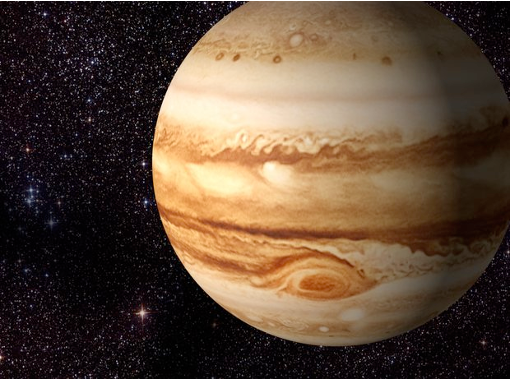
\includegraphics[width=\linewidth]{lectures/figures/0.3_Jupiter_1.png}
                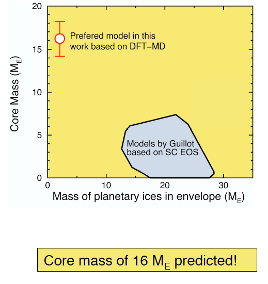
\includegraphics[width=\linewidth]{lectures/figures/0.3_Jupiter_2.png}
            \end{subfigure}
            \begin{subfigure}{0.5\textwidth}
                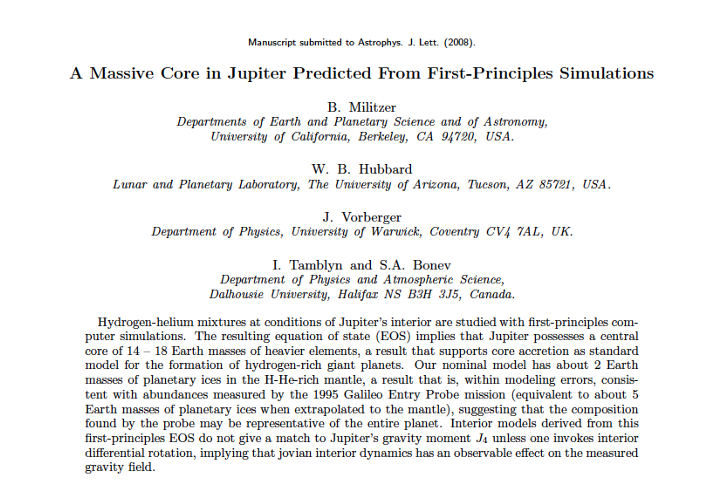
\includegraphics[width=\linewidth]{lectures/figures/0.3_Jupiter_3.png}
            \end{subfigure}
            \caption{Reproduced from ref \cite{militzerMassiveCoreJupiter2008a}.}
        \end{figure}
    \end{frame}


    \begin{frame}{Why QM Modeling? Part 2}
        Absolute control over “experiments”
        \begin{figure}
            \centering
            \begin{subfigure}{0.4\linewidth}
                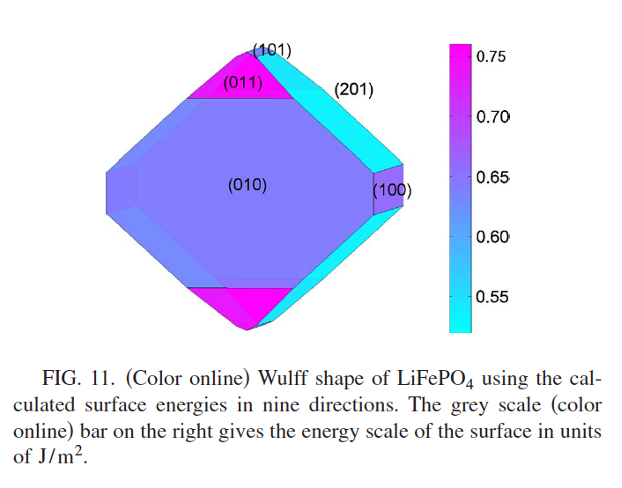
\includegraphics[width=\linewidth]{lectures/figures/0.4_LFP_surface.png}
                \caption{Energy storage.\cite{wangFirstprinciplesStudySurface2007}}
            \end{subfigure}
            \begin{subfigure}{0.2\linewidth}
                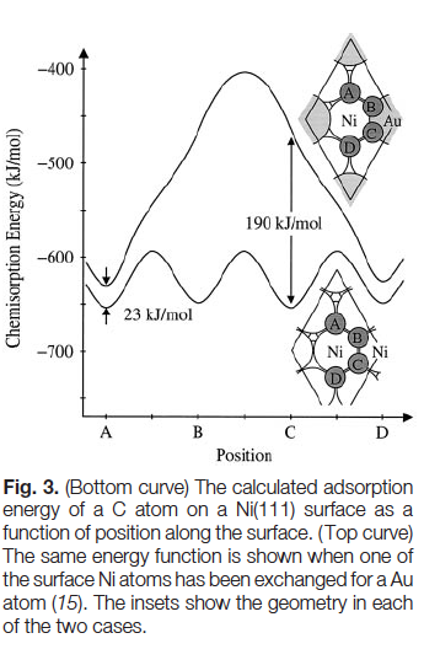
\includegraphics[width=\linewidth]{lectures/figures/0.4_catalysis.png}
                \caption{Catalysis \cite{besenbacherDesignSurfaceAlloy1998}.}
            \end{subfigure}
        \end{figure}
    \end{frame}

    \begin{frame}{Why QM Modeling? Part 3}
        Some things can be done faster... (e.g., materials discovery)
        \begin{figure}
            \centering
            \begin{subfigure}{0.23\linewidth}
                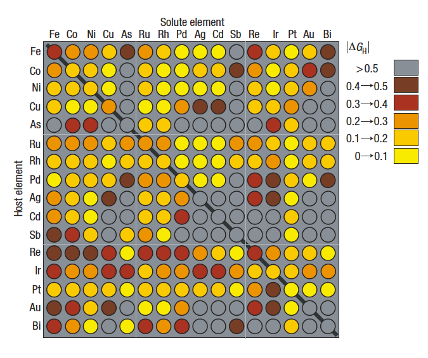
\includegraphics[width=\linewidth]{lectures/figures/0.5_HER.png}
                \caption{Hydrogen evolution\cite{greeleyComputationalHighthroughputScreening2006}}
            \end{subfigure}
            \begin{subfigure}{0.23\linewidth}
                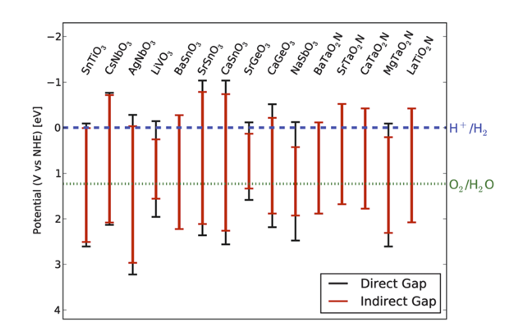
\includegraphics[width=\linewidth]{lectures/figures/0.5_Solar.png}
                \caption{Solar light capture\cite{castelliComputationalScreeningPerovskite2012}.}
            \end{subfigure}
            \begin{subfigure}{0.23\linewidth}
                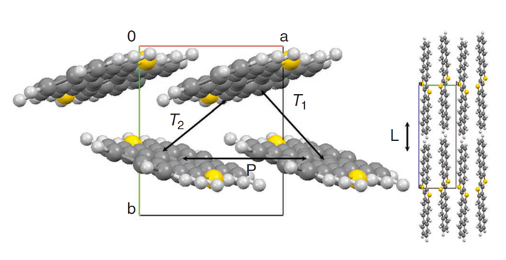
\includegraphics[width=\linewidth]{lectures/figures/0.5_Organic_PVs.png}
                \caption{Organic PVs\cite{sokolovComputationalDiscoveryExperimental2011}.}
            \end{subfigure}
            \begin{subfigure}{0.23\linewidth}
                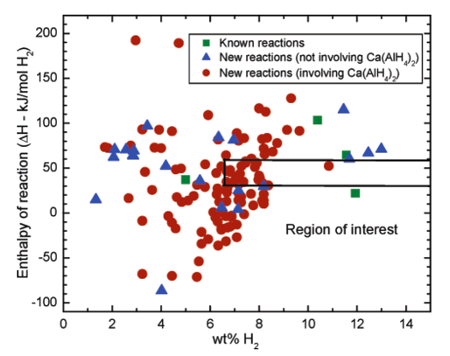
\includegraphics[width=\linewidth]{lectures/figures/0.5_H_storage.png}
                \caption{H storage\cite{alapatiLargeScaleScreeningMetal2008}.}
            \end{subfigure}
        \end{figure}
    \end{frame}


    \begin{frame}{What you will learn in this course}
        \begin{itemize}
            \item Enough QM and theory to understand how to apply them to predict materials properties and solve materials science problems.
            \item Practical aspects of doing simulations, e.g., how do you choose parameters?
            \item Understanding of the limits of what you can do with modeling and where major pitfalls / failures are.
            \item Enough for you to further explore into the big universe of QM modeling (with eyes open).
        \end{itemize}

    \end{frame}

    \begin{frame}{What this course is \textbf{not}}
        \begin{itemize}
            \item A solid-state physics or condensed matter theory course.
            \item A course where you can learn how to write QM code or functionals or pseudopotentials.
        \end{itemize}
    \end{frame}


    \begin{frame}{Instructors}
        \begin{itemize}
            \item Lecturer: Shyue Ping Ong (\href{mailto:ongsp@ucsd.edu}{ongsp@ucsd.edu})
            % \item Teaching Assistant: Keivan Rahmani (\href{mailto:kerahmani@ucsd.edu}{kerahmani@ucsd.edu})
        \end{itemize}
    \end{frame}


    \begin{frame}
        \frametitle{Recommended Textbooks}

        \begin{columns}
            \column{0.5\textwidth}
            \begin{figure}
                \centering
                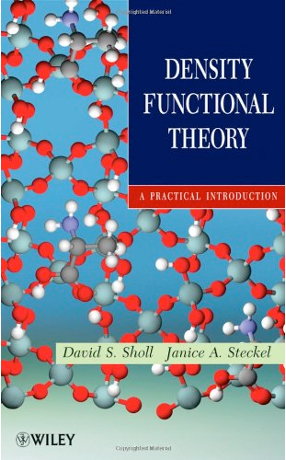
\includegraphics[width=0.4\textwidth]{lectures/figures/0_DFT_a_practical_introduction.png}
                \caption{Density Functional Theory: A Practical Introduction by David Sholl and Janice A Steckel
                \href{https://www.amazon.com/Density-Functional-Theory-Practical-Introduction-ebook/dp/B005PS4Z3A}{[Amazon]}}
            \end{figure}
            \column{0.5\textwidth}
            \begin{figure}
                \centering
                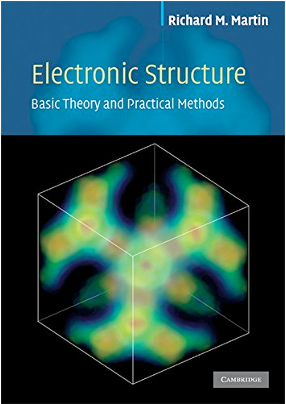
\includegraphics[width=0.4\textwidth]{lectures/figures/0_martin_electronic_structure.png}
                \caption{Electronic Structure: Basic Theory and Practical Methods by Richard M. Martin
                \href{https://www.amazon.com/Electronic-Structure-Theory-Practical-Methods/dp/0521534402 }{[Amazon]}}
            \end{figure}
        \end{columns}
    \end{frame}


    \begin{frame}{Course Structure}
        \begin{itemize}
            \item Lectures/Labs (Tues/Thurs @ 1100-1220) in person.
            \item Note: Please ignore scheduled lab sessions - all labs are held in lecture times, not in a separate time.
            \item Recordings will be available online after the class.
            \item Expectations
            \begin{itemize}
                \item Interactive
                \item Interruptions with questions highly encouraged
                \item Punctuality. Lectures will start exactly on time.
            \end{itemize}
        \end{itemize}
    \end{frame}


    \begin{frame}{Lab Assessment Criteria}
        \begin{table}[]
            \centering
            \footnotesize
            \begin{tabular}{|c|m{4cm}|p{6cm}|c|}
                \hline
                Lab No. & Topic & Objectives & \% \\
                \hline
                1 & Modelling of molecules with nwchem & Functional and basis set choices, familiarization with Unix, use of HPC resources, limited programming
                & 20\%\\
                2 & Modelling crystalline silicon with pwscf &
                Convergence of calculations wrt various parameters, simple python programming
                &
                20\% \\
                3 & Linking calculations to properties of materials & Calculations of different materials, more complex python programming
                & 20\%\\
                4 & Surface calculations & Calculations of surfaces (important for nanomaterials), consolidate lessons from Labs 1-3.
                & 40\%\\
                \hline
            \end{tabular}
        \end{table}
        \begin{itemize}
            \item \textbf{Collaboration policy}: Working together is highly encouraged, but each student must submit his / her own work.
        \end{itemize}
    \end{frame}

    \begin{frame}{Course Plan (Subject to changes)}
        \begin{table}[]
            \centering
            \begin{tabular}{c| l}
                \textbf{Week} & \textbf{Topic}                         \\
                \hline
                1 (this week) & Introduction to QM                     \\
                2             & Hartree-Fock (HF) and Post-HF Approach \\
                3             & Lab 1                                  \\
                4             & Density functional theory              \\
                5             & Lab 2                                  \\
                6             & QM modeling of periodic structures     \\
                7             & Lab 3                                  \\
                8             & Advanced topics                        \\
                9 \& 10       & Lab 4
            \end{tabular}
        \end{table}

    \end{frame}


    \begin{frame}{Useful knowledge}
        \begin{itemize}
            \item Basic familiarity with Unix
            \begin{itemize}
                \item Navigating between folders.
                \item Viewing and editing text files on a Unix/Linux terminal.
                \item If you do not have this familiarity, you can always google for instructions and the lab handouts will provide fairly detailed guides for the most part. Your TAs and classmates can also help you.
            \end{itemize}
            \item Python programming. We will use python to automate calculations. Again, do not worry if you do not know Python. We will not be doing advanced programming and you can easily pick it up. But some form of prior programming experience (Matlab, C, Java, etc.) helps a bit.
        \end{itemize}
    \end{frame}


    \begin{frame}{Course Admin}
        \begin{itemize}
            \item Canvas for all course admin, including announcements/communications and submission of labs.
            \item \href{https://materialsvirtuallab.github.io/nano266/}{NANO266 Github repository} for all materials, including labs with instructions.
        \end{itemize}
    \end{frame}


    \begin{frame}{Questions and Feedback}
        \begin{itemize}
            \item Questions welcomed at any time during or after lectures
            \item Your \textbf{feedback} is invaluable for shaping the current course as well as future courses.
            \item Email all feedback directly to \href{mailto:ongsp@ucsd.edu}{ongsp@ucsd.edu}.
        \end{itemize}
    \end{frame}

    \begin{frame}[allowframebreaks]{Bibliography}
        \bibliographystyle{unsrt}
        \bibliography{refs}
    \end{frame}



    \begin{frame}
        \Huge{\centerline{The End}}
    \end{frame}

\end{document}

